\chapter{Introduction}
\labch{introduction}

Recent advances and evolution in software development have made software more and more complex.
The reliability of software systems is based on their correctness.
Any failure or vulnerability in software poses a significant risk, potentially threatening human safety and causing financial losses.
Nowadays, with more complex systems, the likelihood of software containing bugs increases.
The effort and cost to fix bugs grow with late detection, \reftab{effort-to-fix} illustrates the relative costs of fixing bugs at different development stages.
Nowadays, software rules safety-critical systems such as nuclear power plants, car engines, airplane control systems, and medical devices.
For system where safety is critical, addressing bugs before deployment is mandatory.


Nowadays, machine learning software has an ever-increasing societal impact by assisting or even automating decision-making in fields such as social welfare, criminal justice, and even health care.
At the same time, a number of recent cases have shown that such software may reproduce, or even reinforce, bias directly or indirectly present in the training data \cite{BuolamwiniGebru2018,KayMatuszek2015,COMPAS,ObermeyerPowers2019}.
In April 2021, the European Commission proposed a first legal framework on machine learning software -- the Artificial Intelligence Act~\cite{ArtIntAct}
--- which imposes strict requirements to minimize the risk of discriminatory outcomes.

Moreover, recent advancements in artificial intelligence have led to the rise of large language models (LLMs) capable of generating software from natural language specifications. Agents like OpenAI's ChatGPT and Google's Gemini are gaining widespread use. Specifically designed for coding, GitHub Copilot assists programmers within IDEs and has over a million subscribers. Despite their benefits, AI-generated code can introduce as many bugs as human-written code, making it crucial to use techniques that detect software errors or certify intended behaviors.

\section{Software Quality}

Software quality is a measure of how well software meets its requirements.
The most common method to ensure software quality is \emph{testing}.
The correct behavior of software is tested empirically for finite number of inputs against a set of assertions that specify the functional requirements of the code.
However, testing has inherent limitations.
Testing can only verify a program against the functional requirements, which may be poorly defined and ambiguous, leading to inadequate testing.
Exhaustive testing of systems is impractical, and constraints on time and budget can further impact the process.
But mostly, testing is not sufficient to guarantee the absence of bugs in software\sidenote{``program testing can be quite effective for showing the presence of bugs, but is hopelessly inadequate for showing their absence.'' -- Edsger W. Dijkstra \cite{Dijkstra1976}}.
While in some cases it is acceptable to deploy software with bugs (and rely on patches to fix them, \reftab{effort-to-fix}), in the case of safety-critical systems, it is necessary to ensure that the software is free of bugs before deployment to avoid catastrophic consequences.

In contrast, \emph{formal methods} provide rigorous mathematical guarantees about the correctness of software.
Thanks to their mathematical foundation, an approach based on formal methods guarantees 100\% accuracy in the verification of software properties.
The idea of formally verifying software is not new, and it has been around since the late 1960s with program proofs and invariants from \sidetextcite{Floyd1967} and \sidetextcite{Hoare1969}.
Even before, formal methods may be traced back to the work of \sidetextcite{Church1936} and \sidetextcite{Turing1936} on the foundations of computation.
According to software engineering practices, formal methods can be introduced early in the development lifecycle, enabling the verification of software properties at the design stage.
%
\begin{center}\em
  Why should formal methods replace other well-known, widely accepted, and user-friendly techniques such as testing?
\end{center}
To answer this question, we provide examples where testing failed.


Ariane 5 rocket failure\sidenote{\url{https://esamultimedia.esa.int/docs/esa-x-1819eng.pdf}} in 1996 caused by an integer overflow bug resulting in a loss of \$370 million.
Airfrance Flight 447 crashed in June 2009, killing hundreds of passengers, due to a probe sensor that were not able to accurately measure the airplane speed, which in turns disengaged the autopilot. The probe fault was not detected during testing as the test engineers assumed that such an event was impossible to happen.
Similarly, the Therac-25 radiation therapy\sidecite{Leveson1993} machine where at least six patients received massive overdoses of radiation due to race conditions.
The Toyota unintended acceleration\sidenote{\url{https://www.embeddedrelated.com/showarticle/1574.php}} case where a stack overflow resulted in the death of 89 people and a lawsuit of \$1.2 billion.
The roundoff error in the Patriot missile system\sidenote{\url{https://www.ima.umn.edu/~arnold/disasters/patriot.html}} that caused the death of 28 people during the Gulf War.
All these cases could have been avoided with formal methods.

Unlike testing, formal methods enable exhaustive investigation and detection of bugs that testing may miss. The actual system requirements are translated into formal specifications, which are mathematically verified to ensure the system's behavior aligns with real-world scenarios.
However, Rice's undecidability theorem \sidecite{Rice1993} states that all non-trivial properties\sidenote{
  A property is non-trivial if it is not true for all programs or false for all programs.
} are undecidable, which means that there is no terminating algorithm that can decide whether a program satisfies a non-trivial property.
Therefore, as a consequence of Rice's theorem, formal methods either sacrifice \emph{completeness}, \emph{soundness}, or \emph{automation}.
Current formal methods can be classified into three categories\sidecite{Cousot2010}: \emph{theorem provers}, \emph{model checking}, and \emph{static analysis}.



\begin{marginfigure}
  \centering
  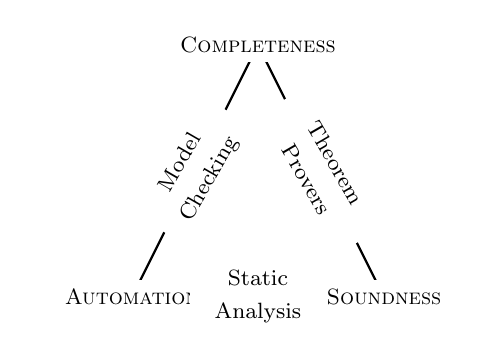
\begin{tikzpicture}[scale=0.8]
    % Draw the triangle
    \draw[thick] (0,0) -- (4,0) -- (2,4) -- cycle;

    % Place the vertices with blue squared borders
    \node[draw, fill=white, text width=2.4cm, align=center, draw=white] at (0,0) {\footnotesize \textsc{Automation}};
    \node[draw, fill=white, text width=2cm, align=center, draw=white] at (4,0) {\footnotesize \textsc{Soundness}};
    \node[draw, fill=white, text width=2.6cm, align=center, draw=white] at (2,4) {\footnotesize \textsc{Completeness}};

    % Place the edges' labels inside the edges
    \node[fill=white, text width=1.5cm, align=center] at (2,0) {\footnotesize Static Analysis};
    \node[fill=white, text width=1.5cm, align=center, rotate=60] at (1,2) {\footnotesize Model Checking};
    \node[fill=white, text width=1.8cm, align=center, rotate=-60] at (3,2) {\footnotesize Theorem Provers};
\end{tikzpicture}
  \caption{Trade-offs in formal methods.}
  \labfig{formal-methods-trade-offs}
\end{marginfigure}

Theorem provers produce proofs of correctness employing interactive tools, also called proof assistants, such as Coq, Isabelle, and HOL Light, or automatic ones like \dots
Ultimately, user interaction is required to guide the proof search.
Even in automatic theorem provers, where automation is key design, to verify any general property, user interaction is required at some point.
Theorem provers are complete and sound, but they are not fully automated.

Formal methods based on model checking explore completely and automatically the state space of a program's model to verify whether undesirable states are reachable.
\sidetextcite{Clarke2004} apply model checking to prove the correctness of ANSI-C programs.
However, model checking-based methods are limited by the state explosion problem: since the number of feasible execution paths grows exponentially with the size of the model, this category of formal methods trade soundness for completeness and automation.

Static analysis is a category of formal methods that analyze without user interaction the program source code to some level of abstraction.
This abstraction is sound but incomplete, meaning that the analysis may report \emph{false alarms}, \ie, warnings that a correct program may be incorrect. However, whenever the static analysis certifies the absence of a bug, the program is indeed bug-free.
The most common static analysis techniques are based on \emph{abstract interpretation}.

Abstract Interpretation \sidecite{Cousot1977} is a general theory for approximating the program semantics, developed by Patrick and Radhia Cousot in the late 1970s.
Their framework is based on the observation that to reason about program properties, not all the computational details are necessary.
Instead, the program's semantics can be approximated by a simpler, more abstract model that facilitate the automatic reasoning.

Over the past decade, abstract interpretation-based static analyses have been successfully applied to the development cycle of real-word software.
The \emph{Astrée} static analyzer \sidecite{Cousot2005} is routinely used to ensure the absence of runtime errors in embedded synchronous C programs for the Airbus A340 and A380.

We provide a formal introduction to abstract interpretation in \refch{abstract-interpretation},
and we recall the main results used in this thesis, which are later illustrated
on a small idealized programming language at the end of the same chapter.


\section{Input Data Usage}

This thesis steams from

\section{Quantitative Properties}

Commonly, in the context of properties of programs, a program either satisfies a property or not.
Such qualitative restriction is not sufficient to capture the complexity of real-world requirements.
Consider for instance one of the most fundamental security issues: protecting the confidentiality of sensitive information.
In secure information flow analysis the question is whether a program could leak information about its secrets.
A classic approach, based on any of the formal methods explored above, would try to enforce \emph{noninterference}, certifying that a program reveals no information about its secrets.
Unfortunately, noninterference is too strict for many practical applications.
In the case of a digital election protocol, individual votes should be anonymous, but of course the final result needs to be revealed. A password checker should not reveal the password, but it should reveal whether the password is correct.
These cases represent deliberate violations of noninterference that are necessary for the program to fulfill its purpose.

To address this limitation, one approach is to consider quantitative properties.
The key idea is to accept that a program may violate a property, and compare such violation against a threshold.
Programs are classified as \emph{safe} or \emph{unsafe} based on the degree of violation, thus inducing a classification among programs based on how much safety they provide.

\refch{quantitative-input-data-usage} introduces the formal framework, based on abstract interpretation, to reason about quantitative properties of programs of input data usage.


\section{Contributions and Outline}


\begin{definition}[Validation]
  \labdef{validation}
  \begin{align}
    \labeq{validation}
    \defprogram \satisfies \defproperty \iff \collectingsemantics \subseteq \defproperty
  \end{align}
\end{definition}

\begin{definition}[Collecting Semantics]
  \labdef{collecting-semantics}
  \begin{align}
    \labeq{collecting-semantics}
    \collectingsemanticsnoparam \defeq \{ \dependencysemanticsnoparam \}
  \end{align}
\end{definition}

\begin{definition}[Dependency Semantics]
  \labdef{dependency-semantics}
  \begin{align*}
    \dependencysemanticsnoparam \DefeQ \setdef{\inputoutputtuple{\defseq}}{\defseq\in\tracesemanticsnoparam}
  \end{align*}
\end{definition}
